\documentclass[signature=data]{physicsreport}
\usepackage{graphicx}

%%
%% User settings
%%

\classno{}
\stuno{}
\groupno{}
\stuname{}
\expdate{\expdatefmt\today}
\expname{分光计的调节和应用}

%%
%% Document body
%%

\begin{document}
% First page
% Some titles and personal information are defined in ``\maketitle''.
\maketitle
% \section{实验目的}
\section{实验预习}
\newpage

\section{实验现象及数据记录}
% Teacher signature
\makeatletter
\physicsreport@body@signature{data}
\makeatother

\newpage

% Data process and others


\section{数据处理}

\begin{enumerate}
    \item 分别计算相应三种颜色的光(绿光、黄光1、黄光2)在衍射级次k=1、2、3时波长的测量值λk,并计算波长平均值$\overline \lambda$,将$\overline \lambda$与汞灯波长的标准值相比较,计算测量的相对误差。要求写出完整的计算过程,包括所用公式和代入实验数据后的表达式。
    
    衍射角的计算公式为:

    $$\psi_k=\frac{(\theta_1-\theta_1^\prime)+(\theta_2-\theta_2^\prime)}{4}$$

    波长的计算公式为:

    $$\lambda_k=\frac{d\sin\psi_k}{k}$$

    计算结果如下:

    % Please add the following required packages to your document preamble:
% \usepackage{multirow}
% Please add the following required packages to your document preamble:
% \usepackage{multirow}
\begin{table}[h]
    \centering
    \begin{tabular}{|c|c|c|c|c|c|}
    \hline
    颜色                 & 衍射级次 $k$ & $\lambda_k(nm)$ & 波长平均值 $\overline{\lambda}(nm)$ & 标准波长(nm)           & 相对误差         \\ \hline
    \multirow{3}{*}{绿} & 1                                                  & 543.94          & \multirow{3}{*}{546.78}        & \multirow{3}{*}{546.1} & \multirow{3}{*}{0.124\%} \\ \cline{2-3}
                        & 2                                                  & 547.08         &                           &                    &                    \\ \cline{2-3}
                        & 3                                                  & 549.32            &                           &                    &                    \\ \hline
    \multirow{3}{*}{黄1}  & 1                                                  & 583.12            & \multirow{3}{*}{578.11}         & \multirow{3}{*}{577.0}  & \multirow{3}{*}{0.193\%}  \\ \cline{2-3}
                        & 2                                                  & 578.11            &                           &                    &                    \\ \cline{2-3}
                        & 3                                                 & 573.10            &                           &                    &                    \\ \hline
    \multirow{3}{*}{黄2} & 1                                                 & 586.70            & \multirow{3}{*}{568.12}         & \multirow{3}{*}{579.1}  & \multirow{3}{*}{1.896\%}  \\ \cline{2-3}
                        & 2                                                 &  580.04           &                           &                    &                    \\ \cline{2-3}
                        & 3                                                 &  537.62           &                           &                    &                    \\ \hline
    \end{tabular}
\end{table}
    
    
    \item 计算衍射光栅对黄光1和黄光2在衍射级次k=1、2、3时的角色散率$D_k$。
    
    角色散率的计算公式为:

    $$D_k=\frac{k}{d\cos\psi_k}$$

    计算结果如下:

    \begin{table}[H]
        \centering
        \begin{tabular}{|c|c|c|}
        \hline
        颜色                 & 衍射级次 $k$ & $D_k(mm^{-1})$          \\ \hline
        \multirow{3}{*}{黄1}  & 1                 & 304.70              \\ \cline{2-3}
                            & 2                   & 639.72                 \\ \cline{2-3}
                            & 3                   & 1050.52                  \\ \hline
        \multirow{3}{*}{黄2} & 1                  & 304.76              \\ \cline{2-3}
                            & 2                  & 640.01                  \\ \cline{2-3}
                            & 3                  & 1028.40                    \\ \hline
        \end{tabular}
    \end{table}

    \item 计算三棱镜的顶角、绿光对应的最小偏向角,计算三棱镜材料对绿光的折射率,双黄光的折射率测量为选做内容。
    
    计算三棱镜顶角的计算公式为:

    $$A=\pi-\frac{|\theta_1-\theta_1^\prime|+|\theta_2-\theta_2^\prime|}{2}$$

    代入数据计算得到三棱镜顶角为:$A=180^\circ-\frac{|221^\circ20^\prime-341^\circ28^\prime|+|41^\circ20^\prime-161^\circ20^\prime|}{2}=59.93^\circ$

    计算绿光对应的最小偏向角的公式如下:
    $$\delta_{min} =\frac{|\theta_1-\theta_1^\prime|+|\theta_2-\theta_2^\prime|}{2}$$
    代入数据计算得到三棱镜顶角为:$\delta_{min} =\frac{|279^\circ18^\prime-231^\circ20^\prime|+|99^\circ6^\prime-51^\circ40^\prime|}{2}=47.70^\circ$


    计算三棱镜材料对绿光的折射率的公式如下:

    $$n=\frac{\sin(\frac{A+\delta_{min}}{2})}{\sin\frac{A}{2}}$$

    计算得到$n=\frac{\sin(\frac{59.93^\circ+47.70^\circ}{2})}{\sin\frac{59.93^\circ}{2}}=1.62$

\end{enumerate}




\pagebreak
\section{讨论题}

\subsection{应用分光计进行测量之前,应调节到何种状态?}

望远镜聚焦于无穷远,能够接收平行光。其光轴与载物台的转轴垂直,平行光管发射的平行光与望远镜的光轴同轴。


\subsection{按游标原理,读出下图中的角度数。}

\begin{figure}[H]
    \centering
    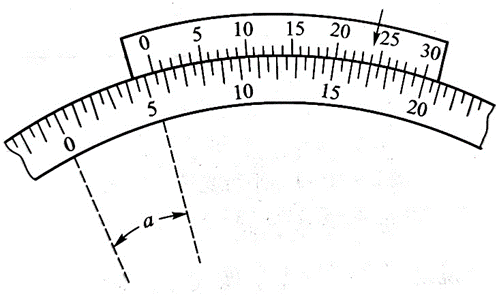
\includegraphics[width=0.5\textwidth]{images/lab14/image.png}
    % \caption{分光计游标读数}
    \label{fig:lab13-fig1}
\end{figure}

根据图片读数为$5^{\circ}24^{\prime}$

\end{document}